\section{Exercise one}

Let's explore the total storage capacity of a system consisting of six disks, each with a capacity of $1\text{ TB}$, under various RAID configurations:
\begin{enumerate}
    \item RAID 0
    \item RAID 1
    \item RAID 01
    \item RAID 10
    \item RAID 5
    \item RAID 6
\end{enumerate}

\subsection*{Solution}
\begin{enumerate}
    \item In RAID 0, all disks are utilized as a single unit:
        \begin{figure}[H]
            \centering
            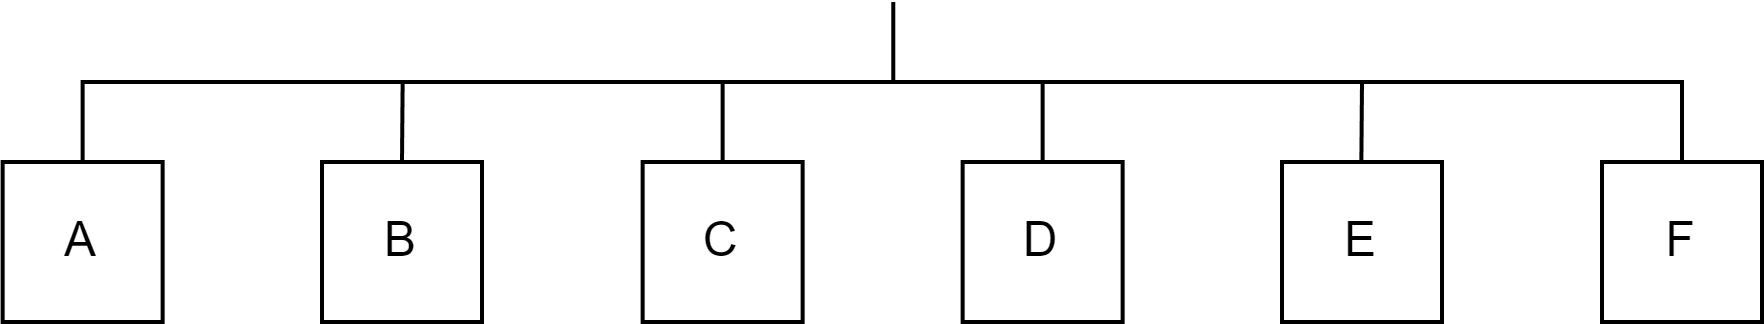
\includegraphics[width=0.7\linewidth]{images/raid0.png}
        \end{figure}
        Hence, the total capacity is the sum of individual disk capacities:
        \[S_C=6\cdot1\text{ TB}=6\text{ TB}\]
    \item RAID 1 duplicates data across disks for high reliability but lower storage:
        \[S_C=1\text{ TB}\]
        \begin{figure}[H]
            \centering
            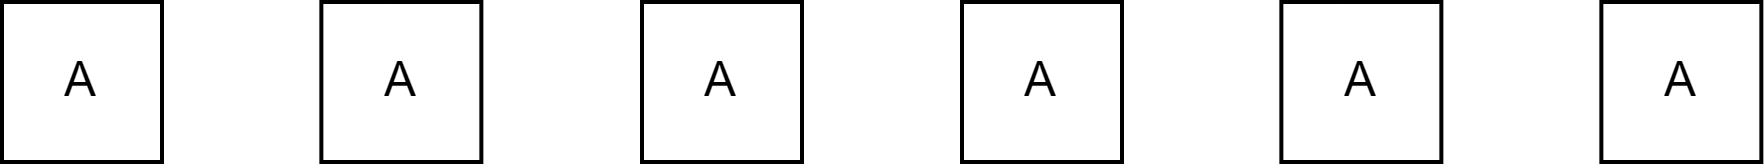
\includegraphics[width=0.7\linewidth]{images/raid1.png}
        \end{figure}
    \item RAID 01 involves striping followed by mirroring, resulting in two sets of mirrored blocks:
        \begin{figure}[H]
            \centering
            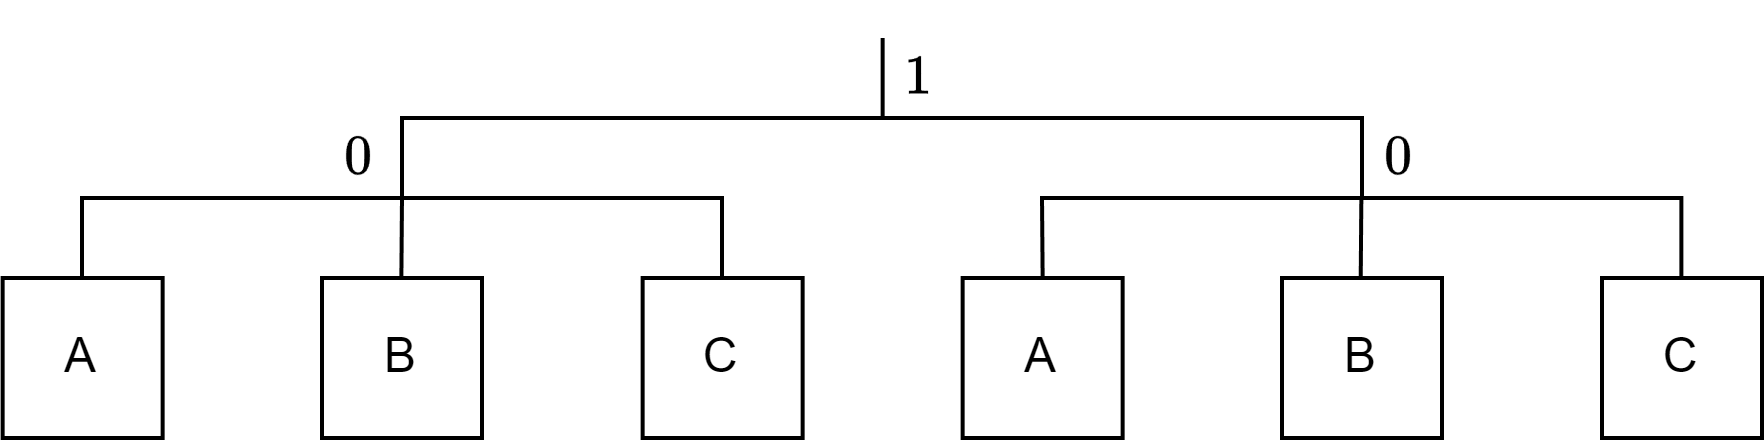
\includegraphics[width=0.7\linewidth]{images/raid01.png}
        \end{figure}
        Thus, the total capacity becomes:
        \[S_C=\dfrac{6}{2}\cdot 1\text{ TB}=3\text{ TB}\]
    \item RAID 10 employs mirroring followed by striping, creating three pairs of mirrored disks:
        \begin{figure}[H]
            \centering
            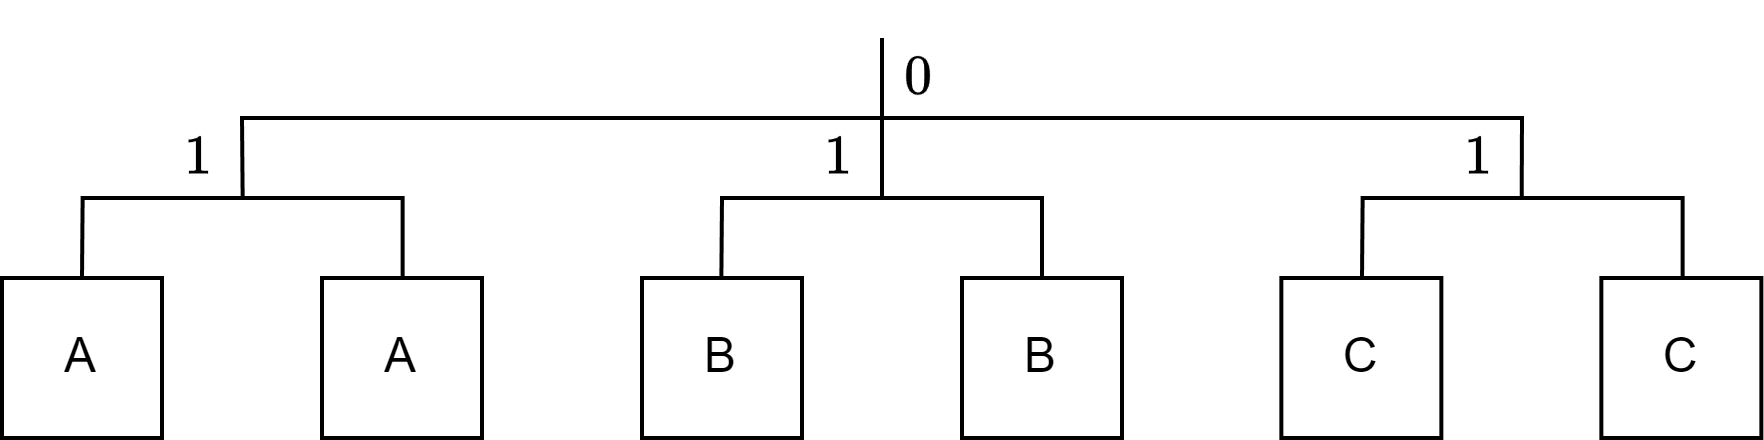
\includegraphics[width=0.7\linewidth]{images/raid10.png}
        \end{figure}
        Therefore, the total capacity is:
        \[S_C=\dfrac{6}{2}\cdot 1\text{ TB}=3\text{ TB}\]
    \item RAID 5 utilizes parity blocks across disks, requiring removal of one disk:
        \begin{figure}[H]
            \centering
            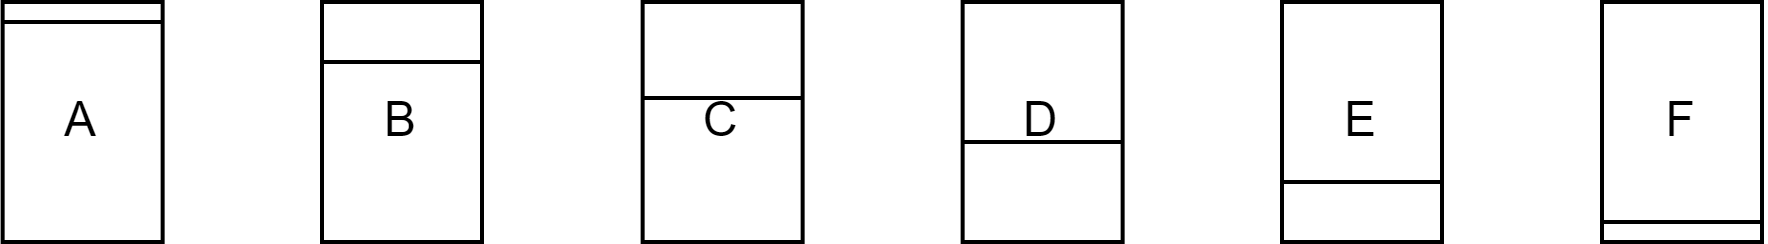
\includegraphics[width=0.7\linewidth]{images/raid5.png}
        \end{figure}
        This yields:
        \[S_C=(N-1)\cdot 1\text{ TB}=5\text{ TB}\]
    \item RAID 6 employs two parity blocks per disk, necessitating removal of two disks:
    \begin{figure}[H]
        \centering
        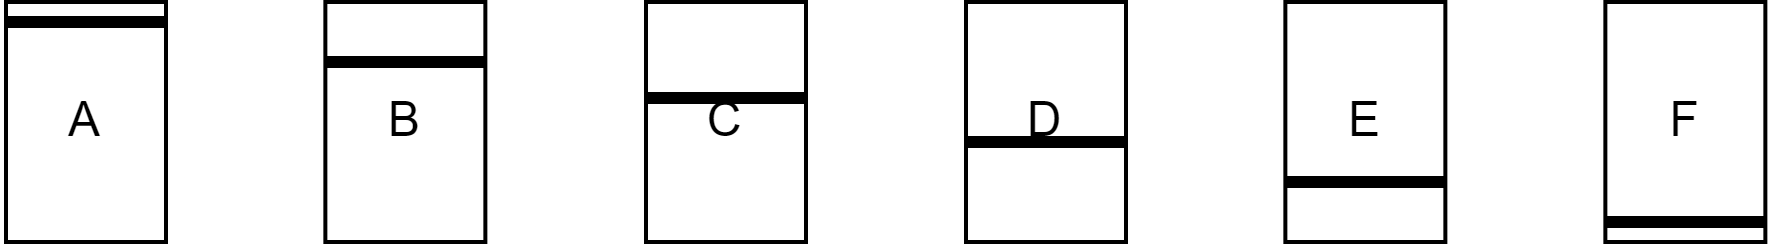
\includegraphics[width=0.7\linewidth]{images/raid6.png}
    \end{figure}
    Resulting in:
    \[S_C=(N-2)\cdot 1\text{ TB}=4\text{ TB}\]
\end{enumerate}
